\begin{figure}[h!]
    \centering
    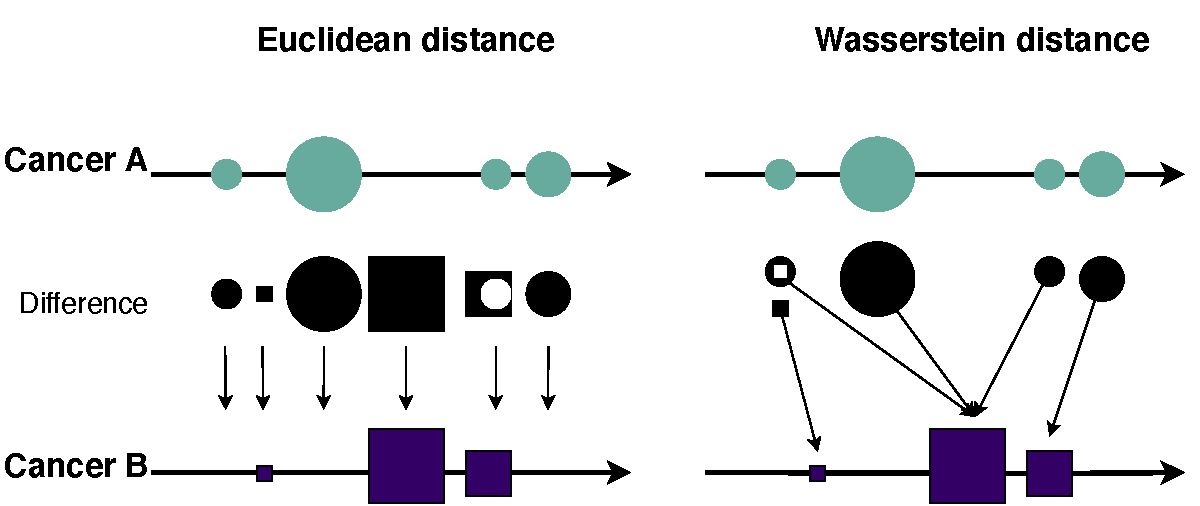
\includegraphics[scale=0.8]{graphics/wasserstein_demo.pdf}
\caption{}
    % \caption{\textbf{Schematic diagram for Euclidean and Wasserstein distance between two vectors.} The green circles are data points on the GLE vector for Cancer A, the purple squares are data points on the GLE vector for Cancer B. The black shapes and the arrows combined represent the difference between Cancers A and B. Euclidean is the point-wise difference between the same location on vectors A and B, and is strictly in the vertical direction. In other words, the Euclidean distance between A and B only depends on how different points of similar coordinates are. Wasserstein takes into account both the vertical and horizontal directions; it is intuitively the minimal amount of work required to transport mass from A to B. The Wasserstein distance between A and B depends on both the difference between the magnitude of data points and the path it takes to move data points from A to B.}
    \label{fig:wasserstein_demo}
\end{figure}
